\documentclass[11pt,a4paper]{article}

\usepackage[utf8]{inputenc}
\usepackage[T1]{fontenc}
\usepackage[spanish,es-tabla,es-noshorthands]{babel}
\usepackage{lmodern}
\usepackage[margin=2.2cm]{geometry}
\usepackage{graphicx}
\usepackage{booktabs}
\usepackage{longtable}
\usepackage{array}
\usepackage{enumitem}
\usepackage[table]{xcolor}
\usepackage{pdflscape}
\usepackage{caption}
\usepackage[hidelinks]{hyperref}

\definecolor{verde}{HTML}{1D5C3A}
\definecolor{verdeclaro}{HTML}{E8F4EC}
\newcolumntype{L}[1]{>{\raggedright\arraybackslash}p{#1}}
\newcolumntype{C}[1]{>{\centering\arraybackslash}p{#1}}
\setlist{nosep,leftmargin=*}
\newenvironment{tabitems}{\begin{minipage}[t]{\linewidth}\begin{itemize}[topsep=0pt,partopsep=0pt]}{\end{itemize}\vspace{4pt}\end{minipage}}
\renewcommand{\arraystretch}{1.3}
\setlength{\parskip}{0.5em}
\setlength{\parindent}{0pt}

\title{\textbf{Laboratorio: Agile Inception del sistema de residuos}\\[0.4em]
\large EcoRuta Cusco: sistema de gestión de recolección de residuos sólidos}
\author{Ingeniería de Software I}
\date{}

\begin{document}
\maketitle

% ---------------------------------------------------------------
\section{Lista de stakeholders}

{\small
\begin{longtable}{L{2.7cm} L{3.6cm} L{4.6cm} C{1.6cm} C{1.3cm}}
\toprule
\textbf{Stakeholder} & \textbf{Rol en el sistema} & \textbf{Intereses / expectativas} & \textbf{Influencia} & \textbf{Interés} \\
\midrule
\endhead
\textbf{Municipalidad} (Gerencia de Medio Ambiente / Limpieza Pública) & Cliente y patrocinador. Planifica rutas, horarios y supervisa el servicio & Reducir costos operativos, mejorar la cobertura, tener datos para tomar decisiones y cumplir la normativa ambiental & Alta & Alto \\
\textbf{Ciudadanos} & Usuarios finales. Consultan horarios, reciben alertas y reportan incidencias & Saber cuándo pasa el camión, que no se acumule basura en las calles y poder reportar problemas fácilmente & Media & Alto \\
\textbf{Operadores de camiones} (choferes y ayudantes) & Usuarios operativos. Siguen las rutas asignadas y registran el avance & Tener rutas claras, una app sencilla y menos reclamos de vecinos & Baja & Medio \\
Supervisores de limpieza pública & Monitorean las rutas en tiempo real y atienden incidencias & Visibilidad de la flota y capacidad de reasignar rutas & Media & Alto \\
Área de TI municipal & Despliega y mantiene el sistema & Que el sistema sea fácil de mantener y seguro & Media & Medio \\
Recicladores formalizados / asociaciones & Recogen residuos reciclables segregados & Acceso a puntos y horarios de reciclaje & Baja & Medio \\
Ministerio del Ambiente / ente fiscalizador & Regulador & Cumplimiento de la Ley de Gestión Integral de Residuos Sólidos (D.L. 1278) & Alta & Bajo \\
\bottomrule
\end{longtable}
}

\textbf{Prioridad de gestión:}
\begin{itemize}
  \item \textbf{Gestionar de cerca:} Municipalidad y supervisores.
  \item \textbf{Mantener informados:} ciudadanos, operadores y recicladores.
  \item \textbf{Mantener satisfecho:} ente regulador.
\end{itemize}

% ---------------------------------------------------------------
\section{Documento de visión}

\subsection{Visión}

\begin{itemize}
  \item \textbf{Para:} la Municipalidad de Cusco y los vecinos del distrito.
  \item \textbf{El sistema:} EcoRuta Cusco, una plataforma web y móvil de gestión de recolección de residuos.
  \item \textbf{Que permite:} planificar y monitorear en tiempo real las rutas de los camiones recolectores, informar a los ciudadanos los horarios de recojo y recibir reportes de acumulación de basura.
  \item \textbf{A diferencia de:} la gestión actual basada en horarios fijos, comunicación informal y sin seguimiento de la flota, que provoca recojos perdidos y puntos críticos de basura.
\end{itemize}

\subsection{Visión extendida}

\begin{quote}
\colorbox{verdeclaro}{\parbox{0.92\linewidth}{\vspace{0.4em}
\textbf{Para} la municipalidad y los ciudadanos del distrito,
\textbf{que necesitan} un servicio de recolección de residuos puntual, predecible y transparente,
\textbf{EcoRuta Cusco es} una plataforma web y móvil de gestión de recolección
\textbf{que} permite planificar rutas, seguir los camiones por GPS, notificar a los vecinos y atender reportes ciudadanos.
\textbf{A diferencia de} la gestión manual actual sin información en tiempo real,
\textbf{nuestro producto} conecta a la municipalidad, los operadores y los ciudadanos en un solo sistema basado en datos.
\vspace{0.4em}}}
\end{quote}

\subsection{Objetivos del proyecto}

\begin{enumerate}
  \item Reducir los recojos no realizados o fuera de horario.
  \item Informar a los ciudadanos con anticipación sobre el paso del camión.
  \item Dar a la municipalidad visibilidad en tiempo real de la flota.
  \item Canalizar los reportes ciudadanos de puntos críticos de basura y medir su tiempo de atención.
  \item Generar reportes para tomar decisiones sobre rutas y recursos.
\end{enumerate}

\subsection{Alcance inicial}

\begin{center}
\begin{tabular}{L{7.6cm} L{7.6cm}}
\toprule
\textbf{Incluye} & \textbf{No incluye} \\
\midrule
Registro de rutas, zonas y horarios & Optimización automática de rutas con IA \\
Seguimiento GPS de camiones desde una app del operador & Sensores de llenado en contenedores (IoT) \\
Consulta de horarios por dirección/zona para ciudadanos & Pagos de arbitrios en línea \\
Notificaciones de ``el camión se acerca'' & Gestión de personal y planillas \\
Reporte ciudadano de basura acumulada (foto + ubicación) & Integración con otros municipios \\
Panel de monitoreo y reportes básicos para la municipalidad & Gestión de residuos industriales u hospitalarios \\
\bottomrule
\end{tabular}
\end{center}

% ---------------------------------------------------------------
\section{Lean Canvas}

La figura~\ref{fig:canvas} muestra el Lean Canvas completo y la tabla~\ref{tab:canvas} detalla cada bloque.



{\small
\begin{longtable}{L{4.2cm} L{11.6cm}}
\caption{Detalle de los bloques del Lean Canvas.}\label{tab:canvas}\\
\toprule
\textbf{Bloque} & \textbf{Contenido} \\
\midrule
\endfirsthead
\toprule
\textbf{Bloque} & \textbf{Contenido} \\
\midrule
\endhead
\textbf{1. Problema} &
\begin{tabitems}
  \item Los vecinos no saben a qué hora pasa el camión y sacan la basura a destiempo.
  \item Se forman puntos críticos de basura en calles y esquinas.
  \item La municipalidad no sabe en tiempo real dónde están los camiones ni si cumplieron la ruta.
  \item Los reclamos ciudadanos se pierden o no se les da seguimiento.
\end{tabitems} \\
\textit{Alternativas existentes} & Horarios fijos comunicados por volantes o redes sociales, el silbato o la campana del camión, reclamos por teléfono o en mesa de partes y control de rutas en hojas de papel. \\
\textbf{2. Segmentos de clientes / Usuarios} &
\begin{tabitems}
  \item \textbf{Cliente:} Municipalidad (gerencia de limpieza pública).
  \item \textbf{Usuarios:} ciudadanos, operadores de camiones y supervisores.
  \item \textbf{Early adopters:} juntas vecinales de zonas con más puntos críticos.
\end{tabitems} \\
\textbf{3. Propuesta de valor única} & ``Que la basura se recoja a tiempo: el ciudadano sabe cuándo pasa el camión y la municipalidad sabe si pasó.'' \\
\textit{Concepto de alto nivel} & ``Como un seguimiento de delivery, pero para el camión de la basura.'' \\
\textbf{4. Solución} &
\begin{tabitems}
  \item App del operador con ruta asignada y envío de ubicación GPS.
  \item App/web ciudadana con horarios, alertas y reportes con foto.
  \item Panel municipal de monitoreo de flota, incidencias e indicadores.
\end{tabitems} \\
\textbf{5. Canales} & Página web y redes sociales de la municipalidad, juntas vecinales, campañas de educación ambiental y códigos QR en contenedores y recibos de arbitrios. \\
\textbf{6. Fuentes de ingreso} & Presupuesto municipal (proyecto de inversión), posible licencia anual del software para otros municipios y fondos o programas ambientales. \\
\textbf{7. Estructura de costos} & Desarrollo y mantenimiento, hosting en la nube, servicio de mapas/GPS, dispositivos móviles para operadores, capacitación y soporte. \\
\textbf{8. Métricas clave} &
\begin{tabitems}
  \item \% de rutas completadas a tiempo.
  \item N.\textsuperscript{o} de usuarios ciudadanos activos.
  \item N.\textsuperscript{o} de puntos críticos reportados vs.\ atendidos.
  \item Tiempo promedio de atención de reportes.
  \item Reducción de reclamos.
\end{tabitems} \\
\textbf{9. Ventaja diferencial} & Adaptado a la realidad local (calles estrechas, zonas sin numeración, conectividad limitada), información en tiempo real y participación ciudadana integrada. \\
\bottomrule
\end{longtable}
}

\begin{landscape}
\begin{figure}[p]
  \centering
  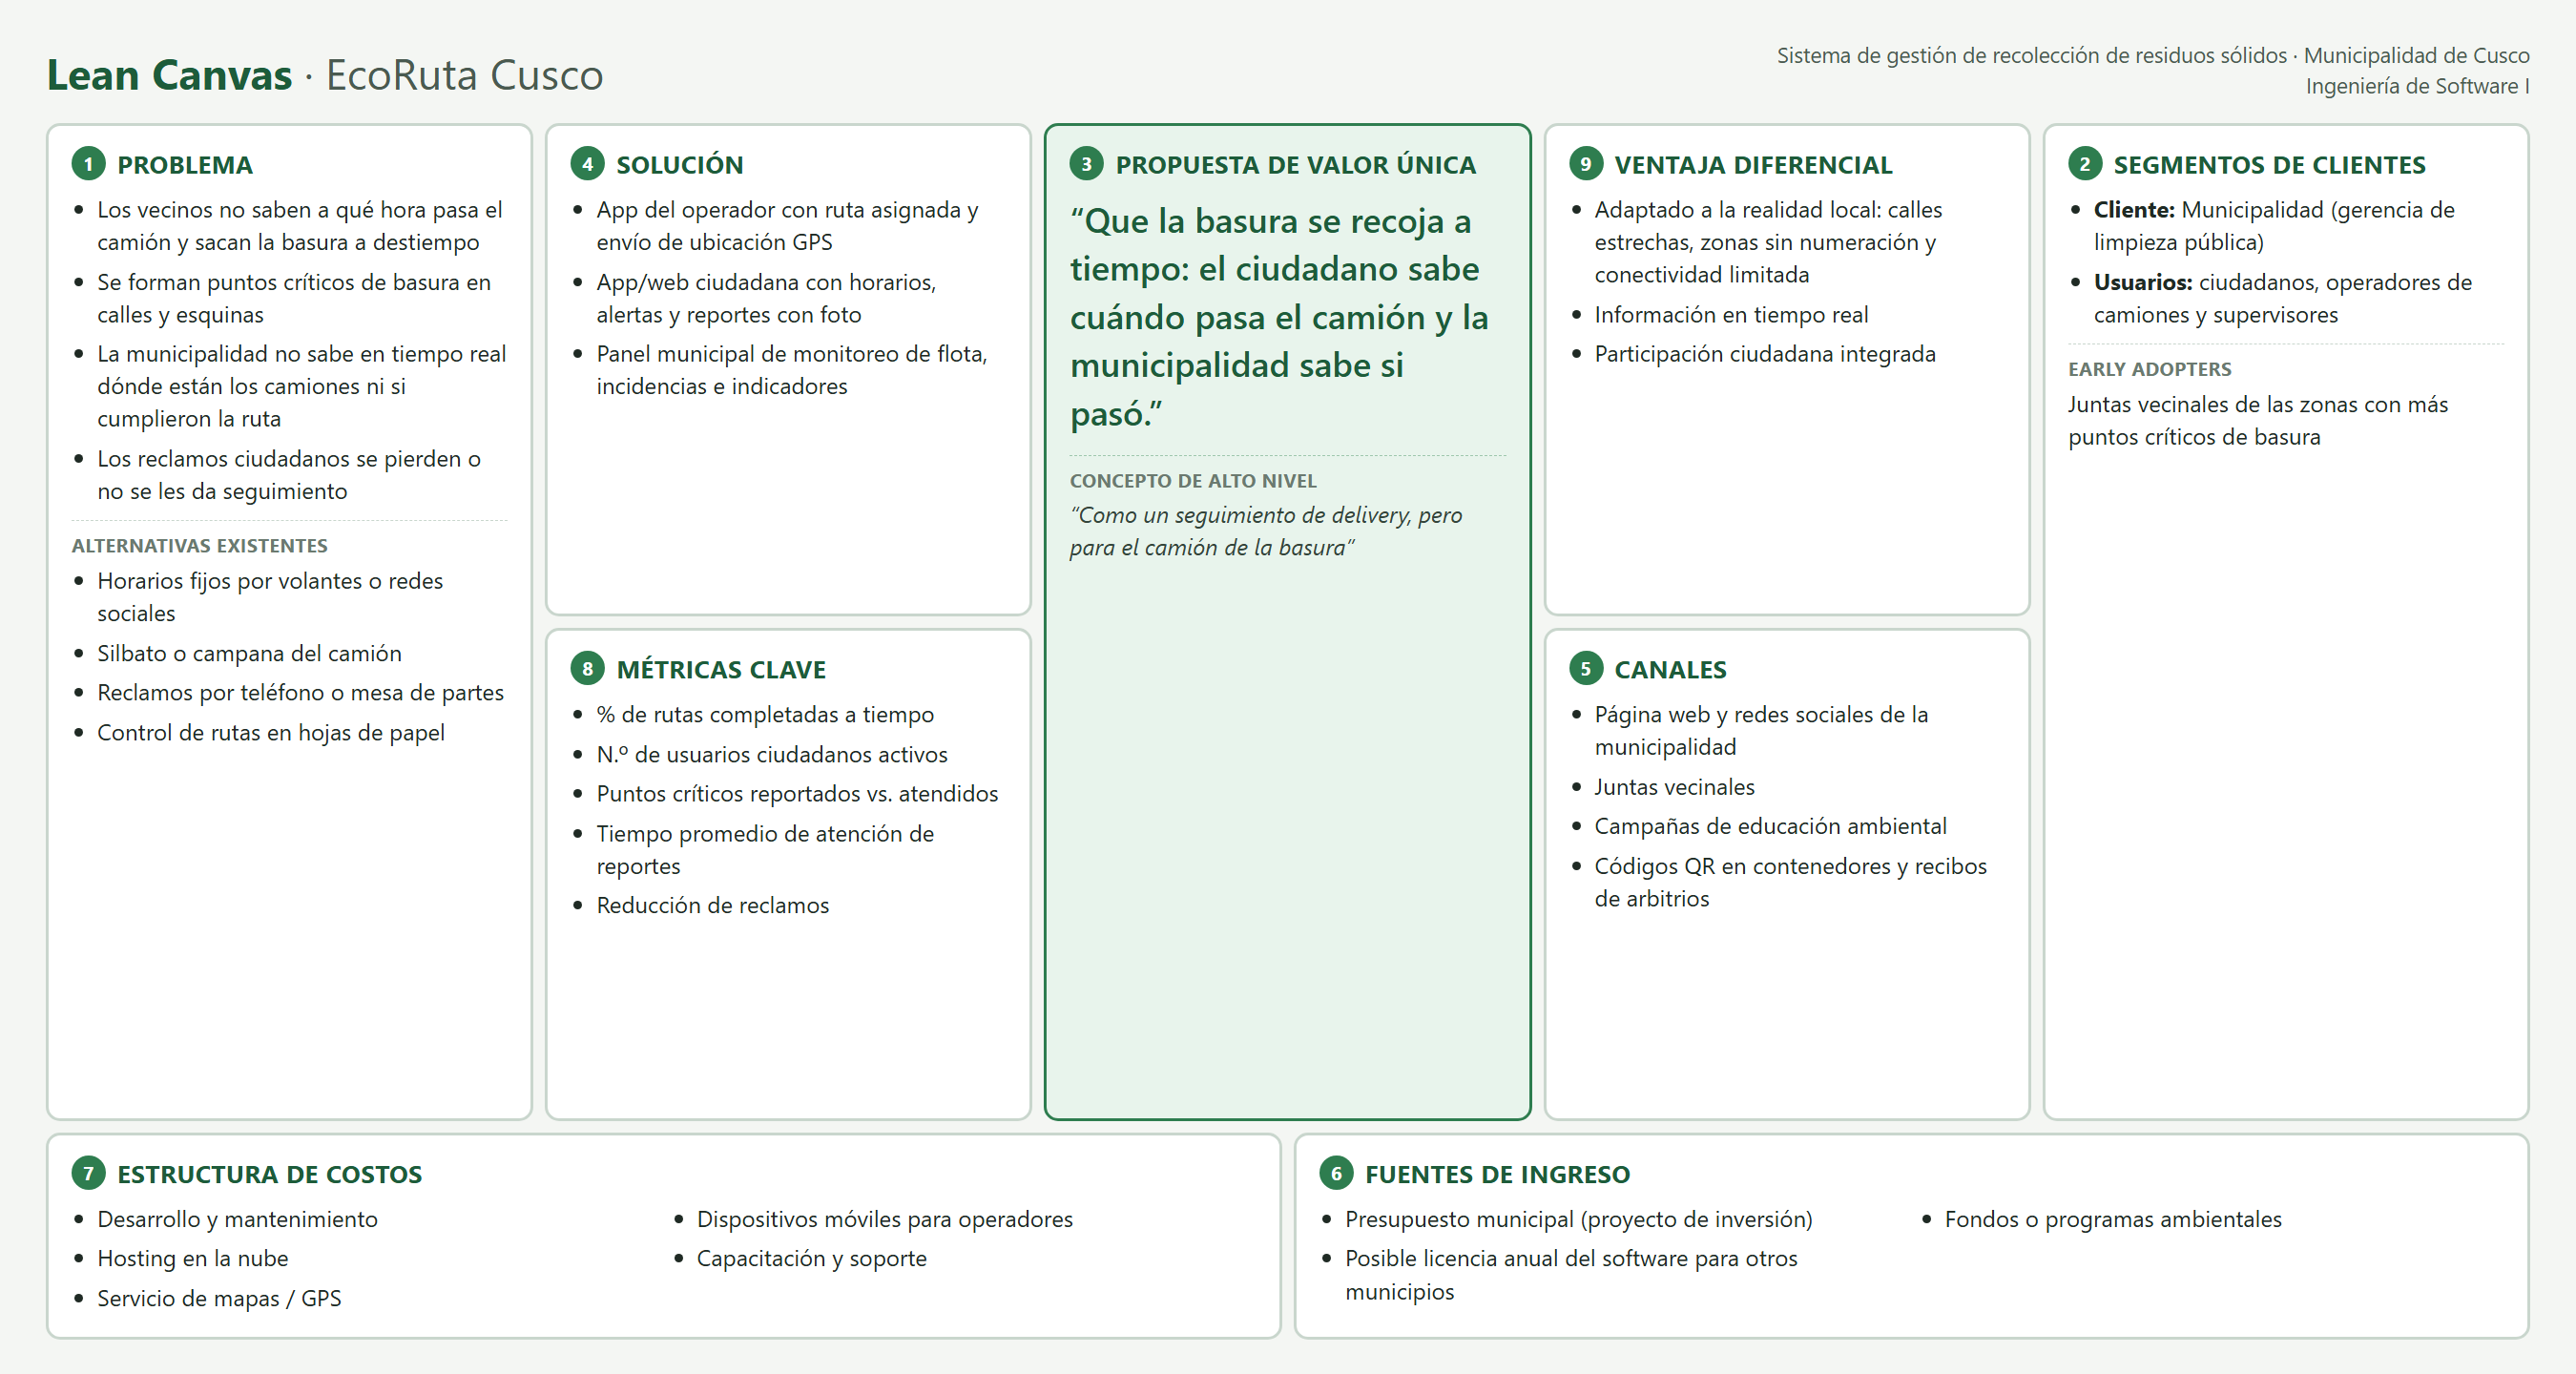
\includegraphics[width=\linewidth]{../img/lean-canvas.png}
  \caption{Lean Canvas de EcoRuta Cusco.}
  \label{fig:canvas}
\end{figure}
\end{landscape}

% ---------------------------------------------------------------
\section{Riesgos iniciales}

Escala: \textbf{A} = alta, \textbf{M} = media, \textbf{B} = baja.

{\small
\begin{longtable}{C{0.8cm} L{3.6cm} L{2.2cm} C{0.9cm} C{1.3cm} L{5.6cm}}
\toprule
\textbf{ID} & \textbf{Riesgo} & \textbf{Categoría} & \textbf{Prob.} & \textbf{Impacto} & \textbf{Mitigación} \\
\midrule
\endhead
R1 & Baja adopción del sistema por parte de los ciudadanos & Negocio & A & A & Campañas con juntas vecinales, interfaz simple y canal alternativo por WhatsApp/SMS \\
R2 & Fallas o pérdida de señal GPS en los camiones & Técnico & M & A & Guardar ubicaciones sin conexión y sincronizarlas después; mostrar la ``última ubicación conocida'' \\
R3 & Resistencia de los operadores a usar la app & Organizacional & M & A & Involucrarlos en el diseño, capacitación práctica y una app con pocos pasos \\
R4 & Conectividad móvil limitada en algunas zonas & Técnico & A & M & Modo offline y bajo consumo de datos \\
R5 & Cambio de gestión municipal o recorte de presupuesto & Político / financiero & M & A & Entregas incrementales con valor visible temprano y documentación de resultados \\
R6 & Direcciones y zonas mal registradas & Datos & M & M & Levantamiento inicial de rutas con el equipo de campo y validación en mapa \\
R7 & Reportes ciudadanos falsos o mal usados & Operativo & M & B & Exigir foto y ubicación, moderación y límite de reportes por usuario \\
R8 & Exposición de datos personales de los ciudadanos & Legal / seguridad & B & A & Cumplir la Ley de Protección de Datos Personales (Ley 29733), recolectar los datos mínimos y cifrarlos \\
R9 & Falta de dispositivos móviles para los operadores & Recursos & M & M & Incluirlos en el presupuesto inicial o usar dispositivos compartidos por camión \\
\bottomrule
\end{longtable}
}

% ---------------------------------------------------------------
\section{Reflexión}

\subsection*{¿Por qué Git es crítico en proyectos colaborativos?}

Porque permite que varias personas trabajen sobre el mismo código al mismo tiempo sin sobrescribirse. Cada cambio queda registrado con su autor, fecha y motivo. Con las ramas, cada integrante puede desarrollar una funcionalidad de forma aislada y luego integrarla mediante \textit{merge} o \textit{pull request}, lo que facilita la revisión. Además, junto con GitHub, sirve como respaldo remoto y fuente única de verdad del proyecto.

\subsection*{¿Qué problemas evita?}

\begin{itemize}
  \item Pérdida de código por sobrescritura o por fallas del equipo.
  \item Confusión de versiones del tipo ``final\_v2\_ahora\_si.zip''.
  \item Conflictos no detectados entre cambios de distintos integrantes.
  \item No poder volver a una versión que sí funcionaba.
  \item No saber quién hizo un cambio ni por qué.
\end{itemize}

Además, en este proyecto también versionamos los artefactos del Agile Inception (visión, canvas y riesgos), así que la evolución del alcance queda trazada junto con el código.

% ---------------------------------------------------------------
\section{Trabajo extra}

\subsection{Refinamiento del Lean Canvas}

\begin{itemize}
  \item Se completaron los \textbf{9 bloques}, no solo los 4 solicitados.
  \item Se separó \textbf{cliente} (quien paga: la municipalidad) de \textbf{usuarios} (ciudadanos y operadores).
  \item Se definieron \textbf{early adopters} para validar el MVP en una zona piloto.
  \item Se agregaron \textbf{métricas medibles} para evaluar el éxito del piloto.
\end{itemize}

\subsection{Soluciones similares}

{\small
\begin{longtable}{L{2.6cm} L{4.8cm} L{3.4cm} L{4.6cm}}
\toprule
\textbf{Solución} & \textbf{Qué ofrece} & \textbf{Qué tomamos como idea} & \textbf{Diferencia con EcoRuta} \\
\midrule
\endhead
\textbf{RUBICON\-Smart\-City} (EE.\,UU.; desde agosto de 2024 pertenece a Routeware) & Software para flotas municipales de recolección: seguimiento GPS de vehículos, avance de rutas en tiempo real, verificación digital del servicio y portal web para supervisores. Usado en ciudades como Atlanta y Denver & Panel de flota y confirmación del servicio por parada & Requiere hardware dedicado en cada camión (tablet, dispositivo telemático y cámara); no está orientado al ciudadano \\
\textbf{Sensoneo} (Eslovaquia) & Sensores ultrasónicos de nivel de llenado en contenedores y software de optimización de rutas. Caso emblemático: Bratislava, con sensores en unos 1\,750 contenedores y equipos en 92 camiones & Planificar las rutas según datos reales (fase futura) & Requiere infraestructura IoT, fuera del alcance del MVP \\
\textbf{Recycle Coach} (EE.\,UU. y Canadá) & App web y móvil gratuita para vecinos: calendario de recojo por dirección, recordatorios (push, SMS o correo), avisos de cambios de horario, buscador de ``¿dónde va cada residuo?'' y reporte de recojos no realizados & Consulta de horarios por dirección y alertas configurables & Trabaja con horarios fijos y no muestra la ubicación real del camión \\
\textbf{SeeClickFix 311 CRM} (EE.\,UU.; producto de CivicPlus) & Plataforma web y móvil para que los vecinos reporten problemas urbanos y sigan su atención; asigna los reportes según ubicación y categoría y detecta duplicados & Reporte ciudadano con ubicación, asignación automática y seguimiento del estado & Es genérica para cualquier servicio municipal y no se especializa en residuos \\
\bottomrule
\end{longtable}
}

{\footnotesize\textit{Fuentes: Waste360, Business Wire y Routeware (Rubicon); sensoneo.com y Recycling Magazine (Sensoneo); páginas municipales de Leduc, Frederick County y Westchester County (Recycle Coach); civicplus.com (SeeClickFix). Consultadas en octubre de 2026.}}

\textbf{Conclusión:} ninguna solución integra en un solo producto de bajo costo el seguimiento de la flota, la información a vecinos y los reportes ciudadanos adaptados al contexto local. Ese es el espacio que busca cubrir EcoRuta Cusco.

\end{document}
